\chapter{Simulation of Reconstruction Algorithm}
This chapter will describe how the system can be mathematically modelled and how the mask for the lensless imager was designed. As mentioned in the previous chapter the system can be modelled as 
\begin{equation}
\label{eq:conv2}
y = \phi * x + e ;
\end{equation}
Ignoring the noise and converting the equation to fourier domain, the equation \ref{eq:conv2} can be re-written as
\begin{equation}
\label{eq:conv3}
F(y) = F(\phi)F(x)
\end{equation}
\begin{equation}
\label{eq:conv3}
F(x) = \frac{F(y)}{F(\phi)}
\end{equation}
\begin{equation}
\label{eq:conv4}
x = F^{-1}(\frac{F(y)}{F(\phi)})
\end{equation}
Equation \ref{eq:conv4} is the simplest possible computational inversion of the scene from the sensor. This method has also been used in \cite{Toeplitz}. As mentioned in the previous chapter, there are two types of masks that can be used for the purpose of encoding the scene onto the mask, namely separable and non-separable mask. MATLAB has been used for the purpose of simulating the algorithms. In this chapter, we would simulate two types of mask patterns, namely separable and non-separable mask patterns. A separable mask pattern is one in which the mask matrix $\phi$ can be expressed in-terms of two sub- matrices:
\begin{equation}
\phi = \phi_L * \phi_R
\end{equation}
Both $\phi_L$ and $\phi_R$ are doubly-toeplitz mask. The mathematical model is also changed as described by the equation \ref{eq:separable}. A non-separable mask is one which does not follow this property and follows equation \ref{eq:conv2}.

\section{Simulation of a non-separable mask}
The non-separable mask simulation was carried out as shown in Figure \ref{fig:non_sep_sim}. Due to the inherent ill-posed mathematics involved in imaging extended scenes, a regularization term is added to the inversion process and we get equation \ref{eq:conv5}. This kind of regularization is called Tikhonov regularization and it regularizes the inversion and controls the effects of noise\cite{Toeplitz}. The same regularization is also used in previous studies\cite{Toeplitz}.

\begin{equation}
\label{eq:conv5}
x = F^{-1}(\frac{F(y)}{F(\phi)+k})
\end{equation}
\begin{figure}[ht]
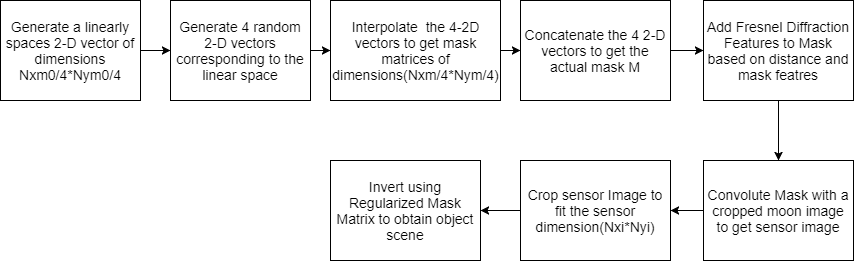
\includegraphics[scale = 0.50]{pics/non_sep_sim_flow}
\caption{Simulation-Flow non-separable mask}
\label{fig:non_sep_sim}
\end{figure}

In order to start with the mathematical modelling process and to imitate the sensor data and reconstruction, a reference image is needed. For that, it was decided to use the full moon image captured by the Apollo 11 space craft\cite{MoonImage}. Since the satellite is going to be pointing towards astronomical objects like the earth, moon, it was decided to crop out a portion of the full moon image as the main purpose of the satellite would be to image specific portions of earth. The simulation is done under the assumption that the camera is enclosed in a box-like structure and light from specific region of the earth/moon would reach it and the sensor size is finite. The image was converted to gray and scaled down form 0 to 1 and is displayed in the \texttt{bone} colormap format available on MATLAB as th colormap would display the minute variations in the reconstructed image. This is illustrated in Figure \ref{fig:moon_image}. The simulation is performed with and without diffraction and analysed. 
\begin{figure}[ht]
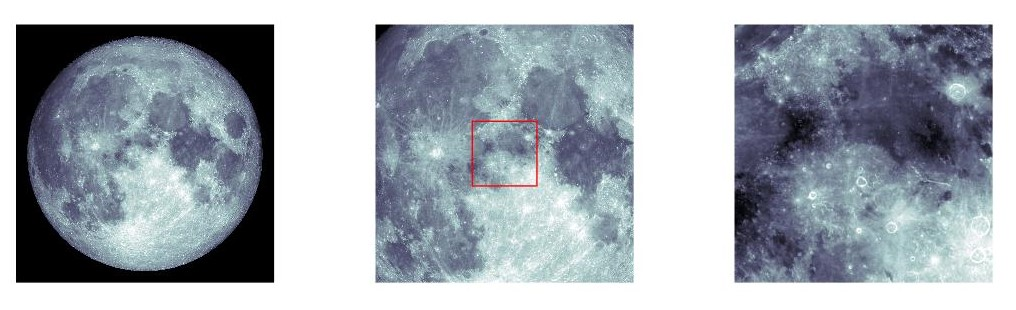
\includegraphics[scale = 0.50]{pics/MoonImagePortion}
\caption{The first image is the orginal image of the moon as taken by Apollo 11 spacecraft. The second image indicates the cropped region and the third image indicates the region that is used for the simulation.}
\label{fig:moon_image}
\end{figure}

\begin{figure}[ht]
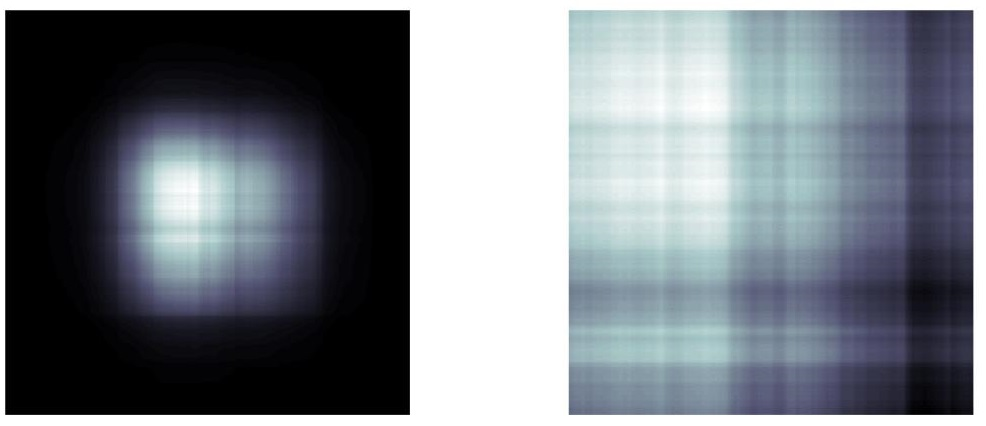
\includegraphics[scale = 0.50]{pics/sensorCropped}
\caption{The first image indicates the sensor image if the sensor plane was infinite. The second image indicates the cropped sensor image that would be formed on an actual finite sensor size(cropped).}
\label{fig:moon_image}
\end{figure}


\section{Simulation of a separable mask}
The non-separable mask simulation was carried out as shown in Figure \ref{fig:sep_sim}.
\begin{figure}[ht]
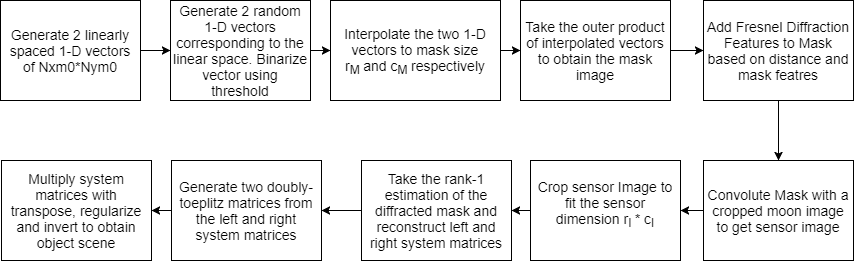
\includegraphics[scale = 0.50]{pics/sep_mask_sim_flow}
\caption{Simulation-Flow separable mask}
\label{fig:sep_sim}
\end{figure}

